\begin{figure}[!htbp]
\caption{Legislator Ideal Points and District Ideology Means}
\begin{centering}
%\centering
%\fbox{
  \begin{tabular}{@{}cc@{}}
	% & & \\  	
  	\small (A) Ideal Point &
    \small (B) Ideal Point  \\
    \small vs Same-Party Share & 
    \small vs Non-Same-Party Share\\
    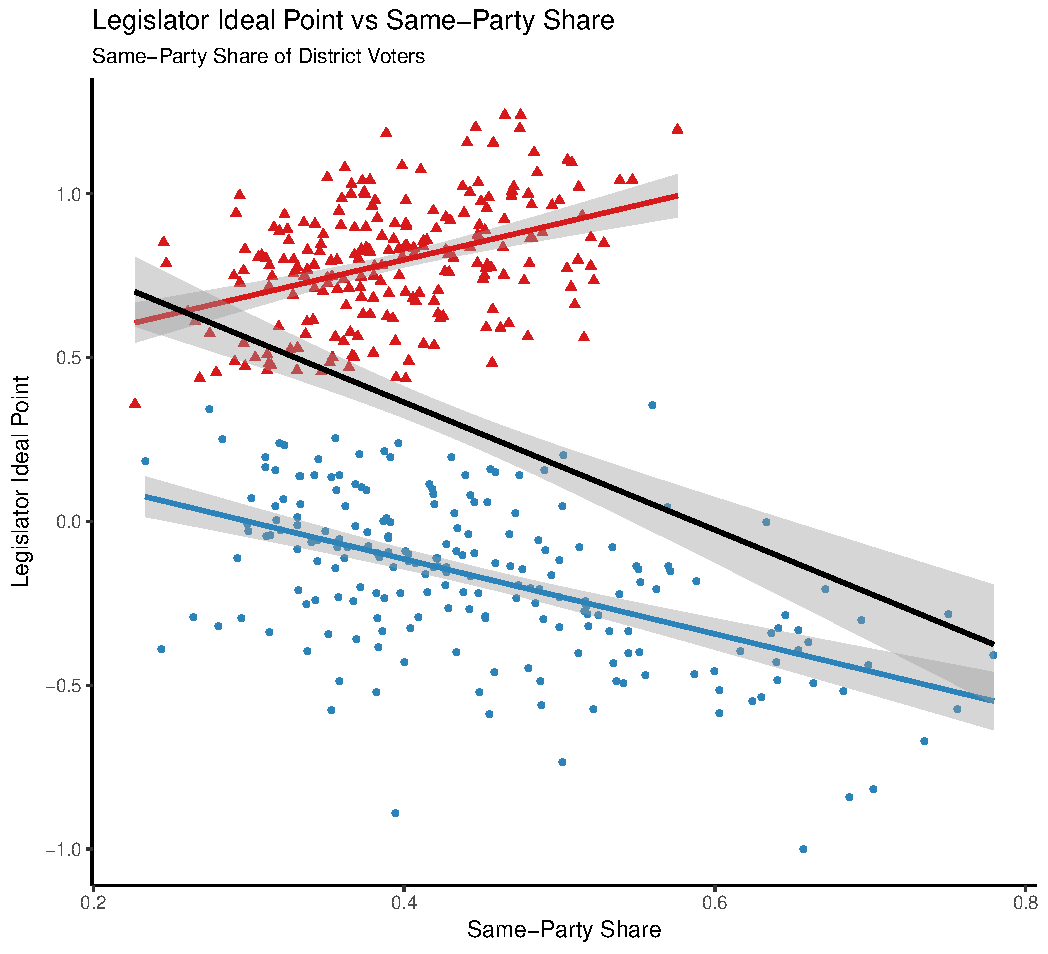
\includegraphics[width=.45\textwidth]{/Users/dsimp/GitHub/Clinton(2006)Rep/drafts/plots/shareplot1.pdf} &
    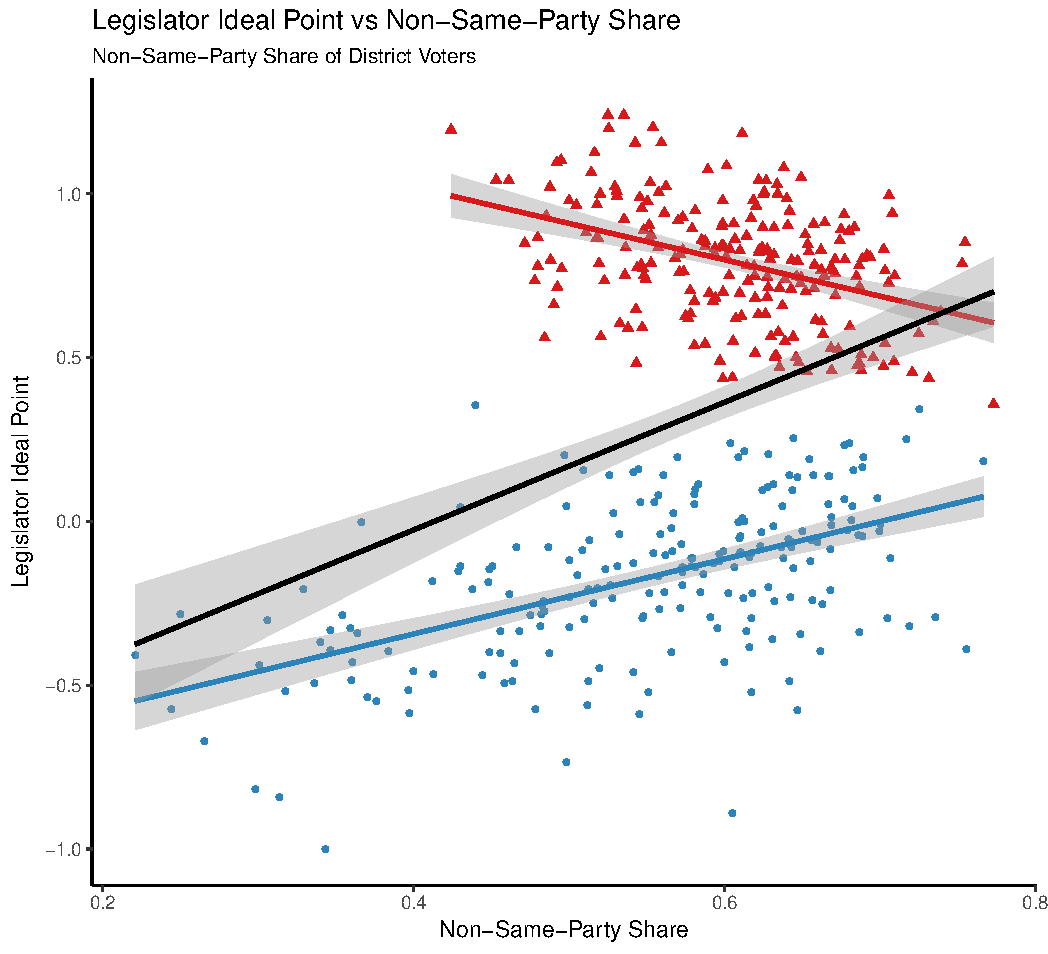
\includegraphics[width=.45\textwidth]{/Users/dsimp/GitHub/Clinton(2006)Rep/drafts/plots/shareplot2.pdf} \\
    % & & \\
    \small (C) Ideal Point & 
    \small (D) Same-Party Ideology\\
    \small vs Opposite Party Share  & 
    \small vs Independent Share\\
    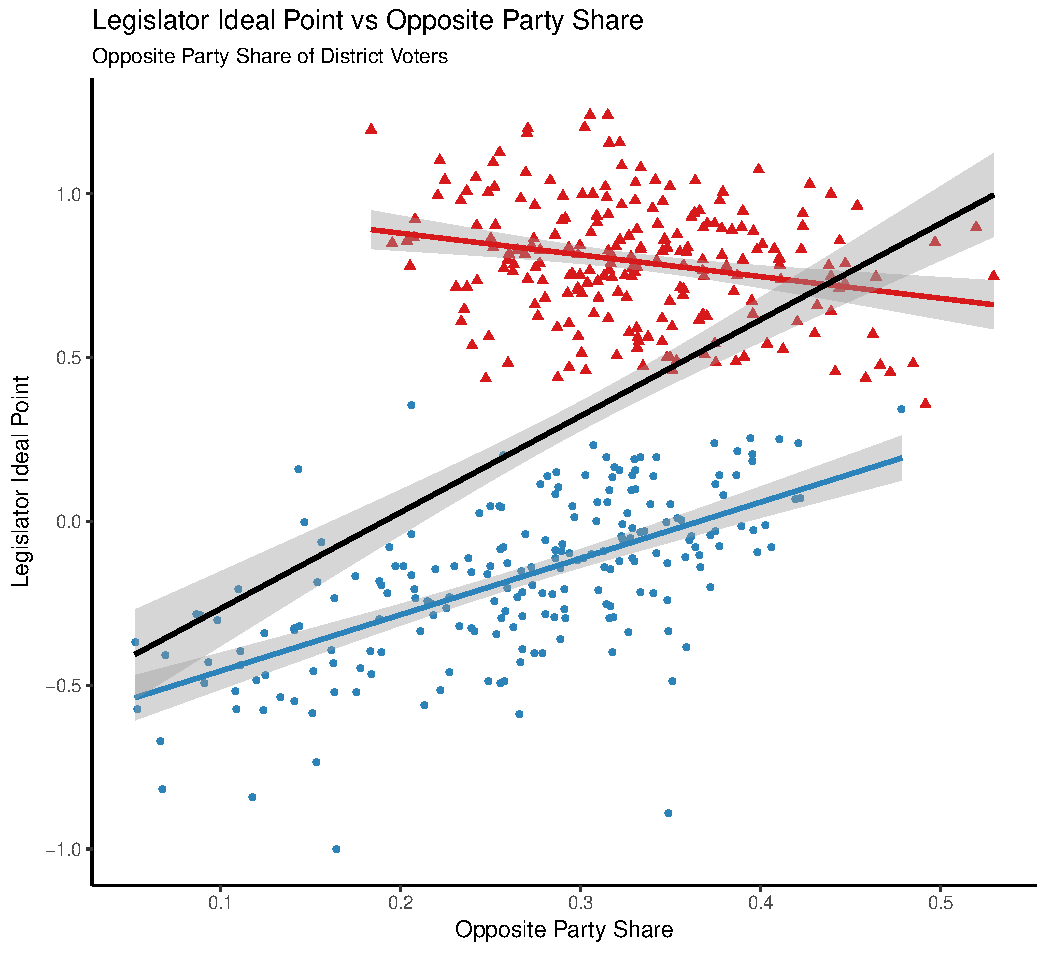
\includegraphics[width=.45\textwidth]{/Users/dsimp/GitHub/Clinton(2006)Rep/drafts/plots/shareplot3.pdf} &
    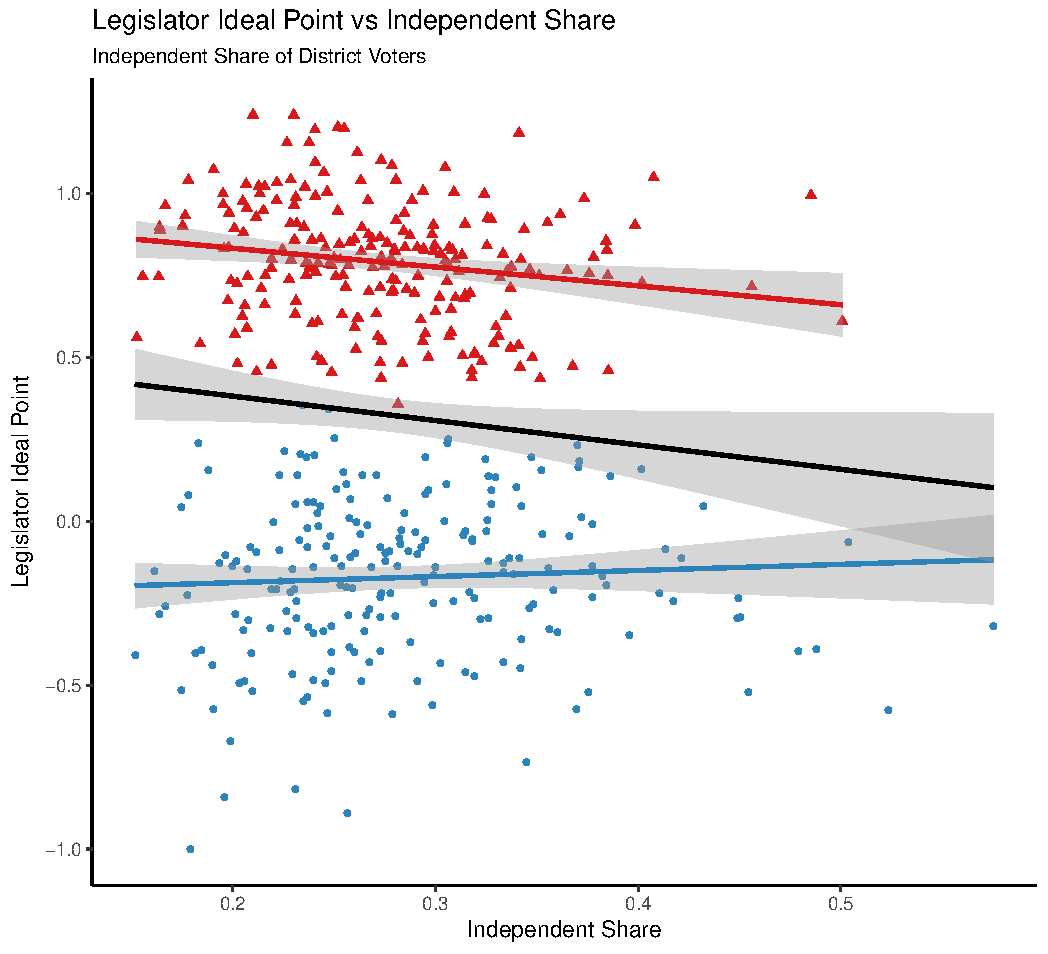
\includegraphics[width=.45\textwidth]{/Users/dsimp/GitHub/Clinton(2006)Rep/drafts/plots/shareplot4.pdf} \\
    % &  &\\
  \end{tabular}
    %}   
 \end{centering}
 \small~~~~~~~~\textbf{Note:} Districts represented by Republicans (Democrats) are plotted with triangles (circles). A bivariate trend line is plotted for overall comparison and party trend lines are plotted for comparison within districts.
\end{figure}.